% Options for packages loaded elsewhere
\PassOptionsToPackage{unicode}{hyperref}
\PassOptionsToPackage{hyphens}{url}
%
\documentclass[
]{article}
\usepackage{lmodern}
\usepackage{amssymb,amsmath}
\usepackage{ifxetex,ifluatex}
\ifnum 0\ifxetex 1\fi\ifluatex 1\fi=0 % if pdftex
  \usepackage[T1]{fontenc}
  \usepackage[utf8]{inputenc}
  \usepackage{textcomp} % provide euro and other symbols
\else % if luatex or xetex
  \usepackage{unicode-math}
  \defaultfontfeatures{Scale=MatchLowercase}
  \defaultfontfeatures[\rmfamily]{Ligatures=TeX,Scale=1}
\fi
% Use upquote if available, for straight quotes in verbatim environments
\IfFileExists{upquote.sty}{\usepackage{upquote}}{}
\IfFileExists{microtype.sty}{% use microtype if available
  \usepackage[]{microtype}
  \UseMicrotypeSet[protrusion]{basicmath} % disable protrusion for tt fonts
}{}
\makeatletter
\@ifundefined{KOMAClassName}{% if non-KOMA class
  \IfFileExists{parskip.sty}{%
    \usepackage{parskip}
  }{% else
    \setlength{\parindent}{0pt}
    \setlength{\parskip}{6pt plus 2pt minus 1pt}}
}{% if KOMA class
  \KOMAoptions{parskip=half}}
\makeatother
\usepackage{xcolor}
\IfFileExists{xurl.sty}{\usepackage{xurl}}{} % add URL line breaks if available
\IfFileExists{bookmark.sty}{\usepackage{bookmark}}{\usepackage{hyperref}}
\hypersetup{
  pdftitle={Measuring the Statistical Performance of Countries: An Overview of the Statistical Performance Indicators and Index},
  pdfauthor={SPI Team},
  hidelinks,
  pdfcreator={LaTeX via pandoc}}
\urlstyle{same} % disable monospaced font for URLs
\usepackage[margin=1in]{geometry}
\usepackage{longtable,booktabs}
% Correct order of tables after \paragraph or \subparagraph
\usepackage{etoolbox}
\makeatletter
\patchcmd\longtable{\par}{\if@noskipsec\mbox{}\fi\par}{}{}
\makeatother
% Allow footnotes in longtable head/foot
\IfFileExists{footnotehyper.sty}{\usepackage{footnotehyper}}{\usepackage{footnote}}
\makesavenoteenv{longtable}
\usepackage{graphicx}
\makeatletter
\def\maxwidth{\ifdim\Gin@nat@width>\linewidth\linewidth\else\Gin@nat@width\fi}
\def\maxheight{\ifdim\Gin@nat@height>\textheight\textheight\else\Gin@nat@height\fi}
\makeatother
% Scale images if necessary, so that they will not overflow the page
% margins by default, and it is still possible to overwrite the defaults
% using explicit options in \includegraphics[width, height, ...]{}
\setkeys{Gin}{width=\maxwidth,height=\maxheight,keepaspectratio}
% Set default figure placement to htbp
\makeatletter
\def\fps@figure{htbp}
\makeatother
\setlength{\emergencystretch}{3em} % prevent overfull lines
\providecommand{\tightlist}{%
  \setlength{\itemsep}{0pt}\setlength{\parskip}{0pt}}
\setcounter{secnumdepth}{5}
\ifluatex
  \usepackage{selnolig}  % disable illegal ligatures
\fi
\newlength{\cslhangindent}
\setlength{\cslhangindent}{1.5em}
\newenvironment{cslreferences}%
  {\setlength{\parindent}{0pt}%
  \everypar{\setlength{\hangindent}{\cslhangindent}}\ignorespaces}%
  {\par}

\title{Measuring the Statistical Performance of Countries: An Overview of the Statistical Performance Indicators and Index}
\author{SPI Team}
\date{2020-10-14}

\begin{document}
\maketitle
\begin{abstract}
Recognizing the new challenges for national statistical systems in monitoring the Sustainable Development Goals (SDGs), the World Bank is developing a new, improved Statistical Performance Indicators (SPI) to monitor progress of the statistical performance of countries. This will replace the Statistical Capacity Index (SCI) the World Bank has regularly published since 2004. This short note briefly discusses the motivation behind the new SPI, describes some of its major features, and discusses a new index based on the indicators.
\end{abstract}

{
\setcounter{tocdepth}{2}
\tableofcontents
}
\hypertarget{motivation}{%
\section{Motivation}\label{motivation}}

The primary purpose of the statistical system is to help users of statistics make better decisions or to hold those decision makers accountable. In the words of Principle 1 of the Fundamental Principles of Official Statistics, the statistics must ``meet the test of practical utility'', serving ``the Government, the economy and the public with data about the economic, demographic, social and environmental situation.''
The national statistical system, or NSS, plays a crucial role in modern economies. It provides stakeholders, ranging from policy makers to stock market analysts and the general public, with the latest data on the country's socio-economic developments. At the international level, monitoring progress on global undertakings such as the recently established Sustainable Development Goals (SDGs) requires high-quality data that must be produced consistently across different national statistical systems. Assessing and improving the capacity of a country's NSS has long been a part of the global agenda. Since the early 2000s, a few capacity assessment tools have been developed to identify the weaknesses and strengths of national statistical systems by other organizations including PARIS21, the Food and Agriculture Organization of the United Nations (FAO), the United Nations Economic Commission for Europe (UNECE), the United Nations Economic Commission for Africa (UNECA), and the U.S. Census Bureau.

The World Bank's Statistical Capacity Index (SCI) is one such tool that has been widely employed. Several international and national agencies have adopted the SCI for measuring progress in statistical capacity building and related investments. The World Bank mainstreamed the SCI in its monitoring and assessment framework and has adopted it as a baseline indicator in various projects at the country level. The SCI is based on publicly available data, and this has various advantages over other indexes of statistical capacity. A key advantage of the SCI is that it can provide assessment of a country's statistical capacity in an internationally comparable and cost-effective manner.

Yet, there are several areas in which the existing SCI can be improved. First, it comprises of a limited number of indicators and includes no indicators of some important data sources, such as labor force surveys, establishment surveys, or administrative data. Second, it ignores the data dissemination practices of an NSS, which is one of the key features of data usage. Third, the SCI has been criticized for placing too much weight on statistical output and activities, while neglecting the infrastructure and resource components of statistical systems. Finally, it is silent on whether the data products produced by the NSS are in high demand.
Since its launch in 2004, the SCI's methodology and coverage have basically remained the same, while the global data landscape has changed significantly. NSSs have made significant advancements with data collection and dissemination practices. At the same time, the adoption of the Sustainable Development Goals (SDGs) set an ambitious development agenda for the next 15 years on ending poverty, protecting the planet, and ensuring prosperity for all by 2030. This, in turn, increased the demand for data and raised the bar for national statistical systems regarding their capacity to produce high-quality data. We thus propose to improve the current SCI to better suit the changing global data landscape.

\hypertarget{overview-of-the-new-spi}{%
\section{Overview of the New SPI}\label{overview-of-the-new-spi}}

The new Statistical Performance Indicators (SPI) builds on the SCI, which the World Bank has regularly published since 2004. Our new SPI will cover many of the same elements as the SCI, such as statistical methodology, source data, and periodicity, but will also expand into new areas. The goals are to offer a framework that was forward looking, measured less mature statistical systems as well as advanced systems, covered the entire national statistical system, not just the National Statistical Office (NSO), and gives countries incentives to build a modern statistical system. We also are committing to making our project open data and open code to build confidence in our work.

The new Statistical Performance Indicators (SPI) are designed to monitor how well countries statistical systems are meeting this purpose. By helping countries and development partners identify the strengths and weaknesses of national statistical systems the SPI can support policy advice for countries about their national statistical systems, investment decisions for donors including the World Bank, benchmarking of national statistical systems, and advocacy for national statistics.

We identify five key dimensions of a country's statistical performance. These are data use, data services, data products, data sources, and data infrastructure . These dimensions can be presented in the form of a dashboard that can help countries identify areas for development in their statistical system. Improvements in performance can be represented as a virtuous data cycle that can become self-sustaining.

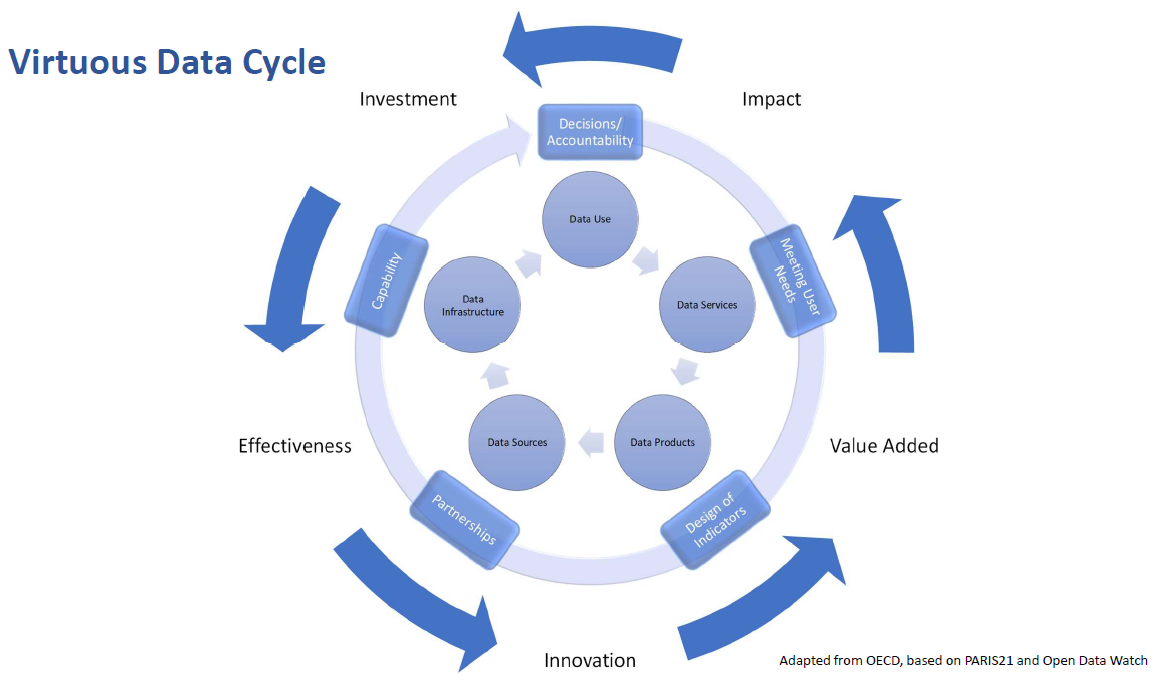
\includegraphics{SPI_cycle.png}

Statistics have no value unless they are used. The first dimension of the Dashboard is therefore data use. A successful statistical system is one that produces data products that are highly used.

In order to meet those needs, the statistical system needs to develop a range of services that connect users and suppliers and facilitate dialogue between them. The second dimension of the SPI is therefore data services that are trusted by users. A successful statistical system is one with highly valued and well used statistical services.

The dialogue between users and suppliers in turn drives the design of statistical products that are to be created including the quality of product needed for the country requirement. This will incorporate accuracy, timeliness, frequency, comparability and levels of disaggregation. The third dimension of the SPI is therefore data products. A successful statistical system is one that generates high quality statistical indicators that can track progress for the Sustainable Development Goals (SDGs).

In order to create the products required, the statistical system needs to make use of a variety of sources from both inside and outside the government. This will include making use of typical data collection methods like censuses and surveys, but also administrative data, geospatial data, and data generated from the private sector and from citizens. The fourth dimension of the dashboard is therefore data sources. A successful statistical system is one which draws on all types of data sources relevant to the indicators that are to be produced.

For the cycle to be complete, capability needs continuously to be reviewed to ensure that it is enough to deliver the products, services and ultimately data use required. The fifth dimension of the SPI is therefore data infrastructure. A successful statistical system is one that develops both hard infrastructure (legislation, governance, standards) and soft infrastructure (skills, partnerships) and has the financial resources to deliver.
The 5 dimensions and associated 22 pillars of the SPI are as shown in Figure 1 below.

\emph{Figure 1: The Dimensions and Pillars that Construct the New SPI}
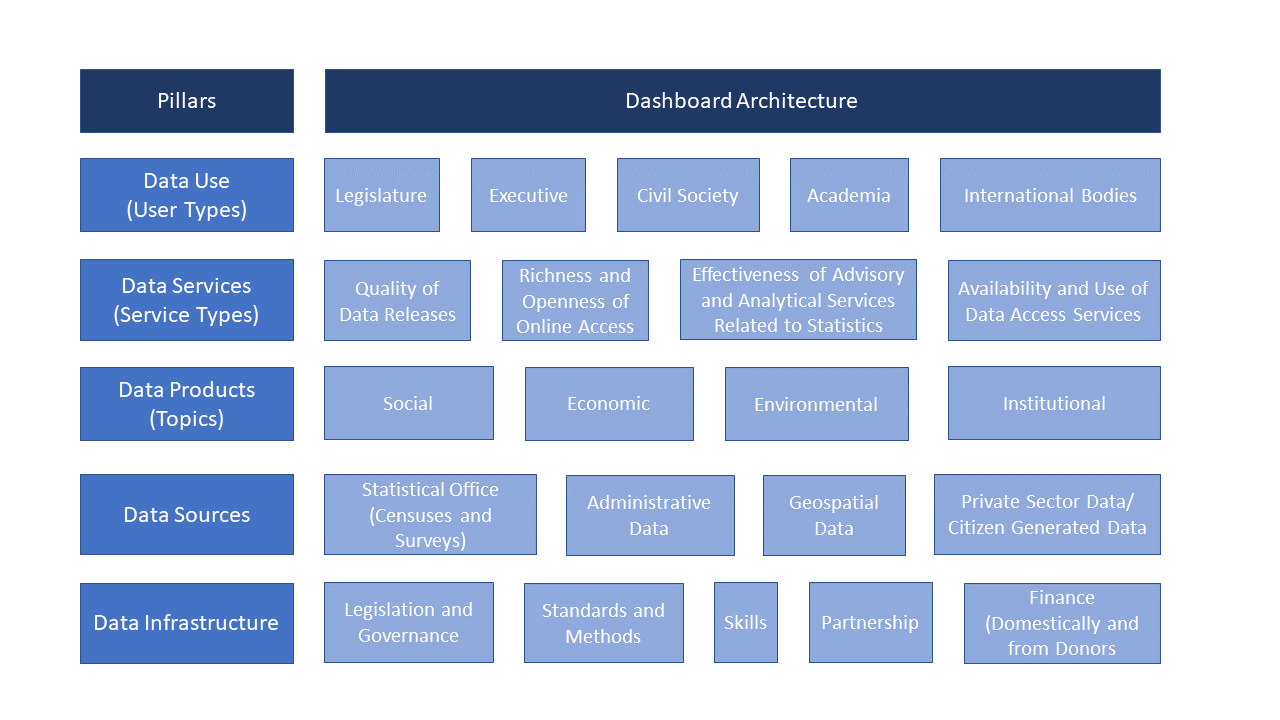
\includegraphics{SPI_dashboard.png}

A score against each element would facilitate:

\begin{enumerate}
\def\labelenumi{\arabic{enumi}.}
\tightlist
\item
  Understanding of the maturity of the national statistical system in relation to others eg quintile groups of countries could be shown against each dimension\\
\item
  This in turn would highlight relative strengths and weaknesses of the system and give an indication of the extent to which the official statistics could be relied upon\\
\item
  It would also point to which other countries the country in question could learn from as it seeks to improve and create incentives to develop in a forward looking rather than backward looking way\\
\item
  Time series would allow assessments to be made of progress of the system and a start point for assessments of return on investment for funding given for capacity building\\
\item
  A dynamic view encouraging continuous improvement. As countries improve the bar for what good looks like would get higher
\end{enumerate}

Key characteristics of the SPI are: (i) uses only publicly accessible data; (ii) transparent methodology; (iii) easily replicable; (iv) provides a long-time series to track progress in performance; (v) captures outcomes and supporting elements; (vi) reflects the SDGs; (vii) facilitates at-a-glance comparisons on a global scale.
We are collecting data on indicators for the 22 pillars above. For dissemination, the SPI will be presented both in the dashboard format above and as an index for each country. Further details on the construction of the new SPI are provided in the remainder of the document.

\hypertarget{pillars-of-the-new-spi}{%
\section{Pillars of the new SPI}\label{pillars-of-the-new-spi}}

A quick primer on names. We refer to the 5 rows in the framework in Figure 1 as dimensions. We refer to the 22 cells in the framwork in Figure 1 as pillars. Finally, each pillar may be composed of multiple indicators. For instance, the pillar on censuses and surveys is made up indicators on whether population censuses have been conducted, agriculture censuses, labor force surveys, etc.

\hypertarget{data-use}{%
\subsection{Data use}\label{data-use}}

The data use dimension is segmented by user type. The tiles on the Dashboard provide an indicator of use of statistics respectively by the legislature, executive, civil society (including sub-national actors), academia and international bodies. A mature system would score well across the tiles. Areas for development would be highlighted by weaker scores in that domain enabling questions to be asked about prioritization amongst user groups and why existing services are not resulting in higher use of national statistics in that segment.

\hypertarget{data-services}{%
\subsection{Data services}\label{data-services}}

The data services dimension is segmented by service type. The tiles on the Dashboard provide an indicator of the quality of data releases, the richness and openness of online access, the effectiveness of advisory and analytical services related to statistics and the availability and use of data services such as secure microdata access. Advisory and analytical services might incorporate elements related to data stewardship services including ethical consideration of proposals and calling out misuse of data in accordance with the Fundamental Principles of Official Statistics.

\hypertarget{data-products}{%
\subsection{Data products}\label{data-products}}

The data products dimension is segmented by topic and organized into social, economic, environmental and institutional domains using the typology of the Sustainable Development Goals. This approach enables comparisons across countries and anchors the system in the 2030 agenda so that a global view can be generated whilst enabling different emphasis to be applied in different countries to reflect the user needs of that country.

\hypertarget{data-sources}{%
\subsection{Data sources}\label{data-sources}}

The data sources dimension is segmented between sources generated by the statistical office (censuses and surveys) and sources accessed from elsewhere (administrative data, geospatial data, private sector data and citizen generated data). The appropriate balance between these types of source will vary depending on the institutional setting and maturity of the statistical system in each country. High scores should reflect the extent to which the sources being utilized enable the necessary statistical indicators to be generated. For example, a low score on environment statistics may reflect a lack of use of (and low score for) geospatial data. This linkage, which is inherent in the data cycle approach, should help highlight areas for investment if country needs are to be met.

\hypertarget{data-infrastructure}{%
\subsection{Data infrastructure}\label{data-infrastructure}}

The data infrastructure dimension is segmented into hard and soft infrastructure segments itemizing essential cross cutting requirements for an effective statistical system. The segments are:

\begin{enumerate}
\def\labelenumi{\arabic{enumi}.}
\tightlist
\item
  Legislation and governance covering the existence of laws and a functioning institutional framework for the statistical system\\
\item
  Standards and methods addressing compliance with recognized frameworks and concepts\\
\item
  Skills including level of skills within the statistical system and amongst users (statistical literacy)\\
\item
  Partnerships reflecting the need for the statistical system to be inclusive and coherent\\
\item
  Finance, both domestically and from donors
\end{enumerate}

\hypertarget{indicators-and-weights}{%
\subsection{Indicators and weights}\label{indicators-and-weights}}

We are seeking answers to the questions:

\begin{enumerate}
\def\labelenumi{\arabic{enumi}.}
\tightlist
\item
  What indicator (that we can measure in practice) could act as a proxy measure for the concept we are trying to capture?\\
\item
  What weight can we assign to the indicator that allows this concept to be aggregated with others in a meaningful way?
\end{enumerate}

There will be no right answer to these questions and the proposed approach makes a virtue of this by:

\begin{enumerate}
\def\labelenumi{\arabic{enumi}.}
\tightlist
\item
  Allowing missing values and setting out how missing values are dealt with for the purposes of making comparisons over time and between countries\\
\item
  Providing users the opportunity to apply their own weights\\
\item
  Releasing the dashboard as a ``Beta'' and encouraging a research agenda to help fill in gaps and improve any elements\\
\item
  Establishing a process for review that enables time series to be respected.\\
\item
  Presenting the dashboard within a toolkit for understanding statistical performance
\end{enumerate}

Below is a brief description of the 22 pillars in our framework. A detailed description of the underlying indicators populating the pillars is also available in the annex.

\includegraphics[width=6.40in,height=7.70in,keepaspectratio]{03_index_files/figure-latex/metadata_tab1-1.png}

\hypertarget{index-methodology}{%
\section{Index Methodology}\label{index-methodology}}

For research purposes, we create an index combining several indicators together to get an overview of country performance. The Index will contain only a subset of the pillars from our framework. For pillars excluded, we either lacked a source with a developed methodology or else the data collection for that measure was incomplete. This is described below:

\begin{itemize}
\item
  \textbf{Pillar 1.1: Data use by national legislature:} \emph{Not included because of lack of established methodology}\\
\item
  \textbf{Pillar 1.2: Data use by national executive branch:} \emph{Not included because of lack of established methodology}\\
\item
  \textbf{Pillar 1.3: Data use by civil society:} \emph{Not included because of lack of established methodology}\\
\item
  \textbf{Pillar 1.4: Data use by academia:} \emph{Not included because of lack of established methodology}\\
\item
  \textbf{Pillar 1.5: Data use by international organizations:} \emph{Reliability/Usefulness of Poverty, Child Mortality, Debt Statistics for international agencies using metadata}
\item
  \textbf{Pillar 2.1: Data Releases:} \emph{SPI.D2.1.GDDS - SDDS/e-GDDS subscription}\\
\item
  \textbf{Pillar 2.2: Online access:} \emph{SPI.D2.2.Openness.subscore ODIN Open Data Openness score}\\
\item
  \textbf{Pillar 2.3: Advisory/ Analytical Services:} \emph{Not included because of lack of established methodology}\\
\item
  \textbf{Pillar 2.4: Data services:} \emph{SPI.D2.4.NADA NADA metadata}
\item
  \textbf{Pillar 3.1: Social Statistics:} \emph{Average score for Goal 1-6 indicators}
\item
  \textbf{Pillar 3.2: Economic Statistics:} \emph{Average score for Goal 7-12 indicators}\\
\item
  \textbf{Pillar 3.3: Environmental Statistics:} \emph{Average score for Goal 13-15 indicators}\\
\item
  \textbf{Pillar 3.4: Institutional Statistics:} \emph{Average score for Goal 16-17 indicators}
\item
  \textbf{Pillar 4.1: Censuses and Surveys:} \emph{Average score Census and Survey Indicators indicators SPI.D4.1\ldots.}
\item
  \textbf{Pillar 4.2: Administrative Data:} \emph{Average score for CRVS indicator. Social Protection, Education, and Labor admin data indicators not included because of lack of established methodolgy. While our team identified several promising sources for administrative data from the World Bank's ASPIRE team, UNESCO, and ILO, incomplete coverage across countries made us drop these indicators from our index. A major research and data collection effort is needed to fill in this information, so that a more comprenhensive picture of administrative data availability can be produced. }\\
\item
  \textbf{Pillar 4.3: Geospatial Data:} \emph{SPI.D4.3.GEO.first.admin.level - Geospatial data available at 1st Admin Level. Although, we view geospatial data availability at the sub-national level as a reasonable proxy for a country's geospatial data capability, and we are using this information in our index, this is another area where more research and efforts on data collection are needed.}
\item
  \textbf{Pillar 4.4: Private/citizen generated data:} \emph{Not included because of lack of established methodology. Currently no comprehensive source exists to measure the use of private and citizen generated data in national statistical systems, and this should be another area where more data collection is needed by the international community.}
\item
  \textbf{Pillar 5.1: Legislation and governance:} \emph{Not included because of insufficient country coverage}\\
\item
  \textbf{Pillar 5.2: Standards and Methods:} \emph{Average score for Standards and Methods indicators SPI.D5.2\ldots.}\\
\item
  \textbf{Pillar 5.3: Skills:} \emph{Not included because of lack of established methodology}\\
\item
  \textbf{Pillar 5.4: Partnerships:} \emph{Not included because of lack of established methodology}\\
\item
  \textbf{Pillar 5.5: Finance:} \emph{Not included because of insufficient country coverage}
\end{itemize}

This process of eliminating some pillars due to lack of established methodology or country coverage results in 12 pillars. This includes 1 on data use, 3 on data services, 4 on data products, 3 on data sources, and 1 on data infrastructure.

\hypertarget{overall-score}{%
\subsection{Overall Score}\label{overall-score}}

Our statistical performance indicators have a three level structure, and our overall score will be formed by sequentially aggregating each level.

To begin we produce a score for each pillar, which is an unweighted average of the indicators within that pillar. For instance, the Census and Surveys pillar will be formed by taking the unweighted average of the Population Census score, the Agriculture Census score, the Business Census score, the Labor Force Survey score, the Health Survey score, etc.

\[ SPI.PILLAR{ctds} = \sum_{i=1}^{N_I} \frac{SPI.IND_{ctdsi}}{N_I} \]

where \(SPI.PILLAR{ctds}\) is pillar s, in dimension d, in time period t, and country c.~\(SPI.IND_{ctdsi}\) is an indicator (e.g.~population census score).

After computing a score for the pillar, we then compute a dimension score, which is the average of the pillars in that dimension. For dimensions 1, 2, 4, and 5, we take the unweighted average of the pillars in the dimension. However, for Dimension 3 on data products, we take a weighted average of the pillars, where the weights are based on the number of SDGs in each pillar (6 SDGs in Pillar 3.1 on social statistics, 6 SDGs in Pillar 3.2 on economic statistics, 2 in Pillar 3.3 on environmental staistics, and 2 in Pillar 3.4 on institutional statistics). We take the perspective that all SDGs are of equal importance, and therefore weight our pillars accordingly.

\[ SPI.DIM_{ctd} = \sum_{s=1}^{N_S} \frac{\omega_{ds} \times SPI.PILLAR{ctds}}{N_S} \]

\(\omega_{ds}\) is the weight for pillar s in dimension d.

After calculating the scores for each dimension The SPI index is the average across the 5 dimensions.

The SPI index is scaled to have a maximum score of 100 and a minimum of 0. A score of 100 would indicate that a country has every single element that we measure in place. A score of 0 indicates that none are in place. To be precise:

\[ SPI.INDEX_{ct} = \sum_{d=1}^{N_D} \frac{SPI.DIM_{ctd}}{N_D} \]

Where SPI.INDEX is the SPI overall index. SPI.DIM are the 5 SPI dimensions listed above. In the notation, c is a country, t is the date, d is a dimension.

The nested structure of our index and the summation methods used to build an overall score ensure the axiomatic properties outlined in (Cameron et al. 2019). These include symmetry, monotonicity, and subgroup decomposability.

\hypertarget{handling-missing-data}{%
\subsection{Handling Missing Data}\label{handling-missing-data}}

For a full description of the methodology behind each specific indicator, please consult the technical documentation. However, we did follow an approach of handling missing values and lining up data, which I will describe in general terms below. For indicators where we had a value for a previous year (say a value in 2018 but not 2019), we would fill in from the previous value. For instance, the open data watch indicators on geo-spatial data was only released in 2018, not 2019, so we filled in the value for 2019 with the value from 2018 as our best estimate of that indicator.

For indicators where we had no data for any years, we chose not to impute a value. In that case, the value for that indicator is null and the country will not have a value for any pillars or dimensions where that value is used.

\hypertarget{process-for-disputing-the-data}{%
\subsection{Process for Disputing the Data}\label{process-for-disputing-the-data}}

Countries will be given an opportunity to dispute the values that make up our indicators. Our team takes every effort to make sure the data presented in ouf Statistical Performance Indicators are accurate, but it is possible that the sources we used to assign values for our indicators are not accurate despite these efforts. Because of this, countries will have a window to provide documentation for any disputed values, and our team will be happy to adjust our scores based on this new information. Precise details for this process will be made available in the future.

\hypertarget{analysis}{%
\section{Analysis}\label{analysis}}

Below we show a set of summary measures for our SPI index. We begin by presenting a world map containing the SPI index values for 2019 for each country. In total, we have 166 countries with sufficient data to compute an index value. This set of countries covers 98.6 percent of the world population.

The map is color coded based on the performance of countries on our index. Given the imprecision inherent in the calculations we recommend that the color coding provides the most detailed subdivisions of maturity. Finer distinctions are unlikely to provide meaningful differentiation between countries.

Countries shaded in dark red are the lowest performing, countries in dark green are the highest performing. Countries are grouped into three groups:

\begin{itemize}
\tightlist
\item
  Low Performers: Countries in the bottom 33\% are classified in this group. Shading is in red. Countries in bottom half of this group are shown in dark red.\\
\item
  Middle Performers: Countries in the middle 33\% are classified in this group. Shading in yellow. Countries in the bottom half of this group are shown in light yellow.\\
\item
  High Performers: Countries in the top 33\% are classified in this group. Shading in green. Countries in the bottom half of this group are shown in light green.
\end{itemize}

\includegraphics{03_index_files/figure-latex/sumstats-1.pdf} \includegraphics{03_index_files/figure-latex/sumstats-2.pdf} \includegraphics{03_index_files/figure-latex/sumstats-3.pdf} \includegraphics{03_index_files/figure-latex/sumstats-4.pdf} \includegraphics{03_index_files/figure-latex/sumstats-5.pdf}

\hypertarget{unique-values}{%
\subsection{Unique Values}\label{unique-values}}

As a check of the data, we calculate the number of unique scores for our SPI index. If our SPI index produces a large number of tied scores, for instance, then our index will be less able to distinguish between the statistical performance of countries. When calculating the number of unique values for 2019, we find that there are 165 unique scores for 166 countries. This means there are 1 tied values. When looking within each dimension.

When looking at each specific dimension, there are only 12 unique scores for Dimension 1 on data use. The data use indicator is coming solely from dimension 1.5 on data use by international organizations. For Dimension 2, there are 158 unique scores. For Dimension 3, there are 164 unique scores. There are 159 unique scores for dimension 4, and there are 19 unique scores for dimension 5.

\hypertarget{relationship-to-gdp-per-capita-and-the-human-capital-index}{%
\subsection{Relationship to GDP Per Capita and the Human Capital Index}\label{relationship-to-gdp-per-capita-and-the-human-capital-index}}

Below, we will present the correlation between our SPI index and the log of GDP per capita and the World Bank's Human Capital Index ((Bank 2020)). The source for GDP per capita comes from the World Bank's World Development Indicators (WDI) database (NY.GDP.PCAP.KD). The GDP per capita numbers are in constant 2010 US\$.

We would expect a strong positive relationship between GDP per capita of countries and their statistical system, as higher income countries would tend to have more resources available for statistical production. In fact, there is a strong relationship between the two. The correlation in 2019 between log GDP per capita and the SPI index is 0.74.\footnote{To understand what effect taking the log has on this correlation, the correlation in 2019 between (non-logged) GDP per capita and the SPI index is 0.64.}

Another measure of a country's development is the Human Capital Index (HCI) developed by the World Bank ((Bank 2020)). The Human Capital Index is designed to capture the amount of human capital a child born today can expect to attain by age 18 in a country. The index combines a country's child mortality, learning adjusted years of schooling, adult survival rates \& stunting into one index. For more details, visit the Human Capital Index website (\url{https://www.worldbank.org/en/publication/human-capital}). Again, we would expect a strong positive relationship between a country's HCI value and their Statistical Performance Indicators index value, as countries with a more developed human capital stock are likely to have greater capacity to produce statistics. Again, this is what we see. The correlation between the 2018 value of the HCI (the latest value available at the time of this writing) and the 2018 value of the SPI index is 0.86.

Below we show the scatter plot of the relationship between log GDP per capita, the HCI, and our SPI index for the years 2016-2019. In general, countries with higher per capita income and higher levels of human capital tend to have better performing statistical systems according to our measure.

\begin{figure}
\centering
\includegraphics{03_index_files/figure-latex/gdp_plot-1.pdf}
\caption{(\#fig:gdp\_plot)~}
\end{figure}

So as to highlight countries where this relationships do not hold as well, the next figure shows the 15 countries that most over-perform and the 15 countries that most under-perform on the SPI Index compared to their levels of GDP per capita and the Human Capital Index. We would not necessarily expect a perfect fit between our SPI index and GDP per capita and the Human Capital Index, as countries differ in the resources put into their statistical system, even conditional on their levels of development. Highlighting outliers can sometimes be a useful exercise for determining whether a measure is identifying on the ground realities.

In order to produce this figure, we estimate an OLS regression of the SPI index in 2019 on log GDP per capita. We then calculate the residual, which can be interpreted as the difference between the country's SPI index value and the expected index value based on their GDP per capita. Countries with values of the residual greater than zero are over-performing based on their GDP per capita and countries with residuals less than zero are under-performing. The corresponding figure for the Human Capital Index is calculated similarly, however in this case we do not take the log, as we did with GDP per capita.

\begin{figure}
\centering
\includegraphics{03_index_files/figure-latex/overperformers-1.pdf}
\caption{\label{fig:overperformers}~}
\end{figure}

\hypertarget{country-changes-in-the-index}{%
\subsection{Country Changes in the Index}\label{country-changes-in-the-index}}

In order to assess how stable our index values are over time, next we will compare the index values in 2016 to the 2019 values. Overall, the SPI index is quite stable over time. The correlation between the 2016 value and the 2019 value is 0.97.

\begin{figure}
\centering
\includegraphics{03_index_files/figure-latex/changes_plot-1.pdf}
\caption{(\#fig:changes\_plot)~}
\end{figure}

While the scores were relatively stable over time, some countries did see large improvements in their score from 2016-2019. The country that improved most on our index from 2016 to 2019 was Myanmar. Myanmar improved by 22.8 points on our scale out of 100. The table below shows the changes in our SPI index for the top 10 largest improvers.

\includegraphics[width=4.80in,height=3.56in,keepaspectratio]{03_index_files/figure-latex/top_bottom_changes_tab-1.png}

\hypertarget{comparison-to-the-statistical-capacity-indicators}{%
\subsection{Comparison to the Statistical Capacity Indicators}\label{comparison-to-the-statistical-capacity-indicators}}

Next, we compare our index to several other indices of statistical performance that have been created. This will provide a sense of how rankings differ across measures, how they correlate with other outcomes, and how the distributions of scores compare.

We compare the SPI index to the older World Bank Statistical Capacity Indicators (\url{http://datatopics.worldbank.org/statisticalcapacity/SCIdashboard.aspx}). The correlation between the SPI index and the SCI is 0.754.

\begin{figure}
\centering
\includegraphics{03_index_files/figure-latex/sci-1.pdf}
\caption{\label{fig:sci}~}
\end{figure}

Next, we show how the relationship to Log GDP per capita differs for the SCI and the SPI index using linear regression. We also include the Open Data Watch and the version of the Statistical Performance Index developed in (Cameron et al. 2019). While showing a strong relationship between an index and log GDP per capita does not mean the index is necessarily correct, and is certainly not necessarily causal, it does provide a face validity check of the index. Heteroskedasticity robust standard errors are shown in the table.

Overall, the new SPI index has the strongest relationship to GDP per capita. The linear regression estimates indicate that a 1\% increase in GDP per capita is associated with a 0.1 point increase in our SPI index score. The r-squared from this regression is 0.49.

\includegraphics[width=6.00in,height=6.43in,keepaspectratio]{03_index_files/figure-latex/sci_spi_reg_tab-1.png}
\includegraphics{03_index_files/figure-latex/sci_spi_reg_tab-2.pdf}

\hypertarget{odin-ranking-comparison}{%
\subsection{ODIN ranking comparison}\label{odin-ranking-comparison}}

We compare the SPI index to the Open Data Watch rankings of country statistical systems (\url{https://odin.opendatawatch.com/report/rankings}). The correlation between the SPI index and the ODIN index is 0.845

\begin{figure}
\centering
\includegraphics{03_index_files/figure-latex/odin-1.pdf}
\caption{\label{fig:odin}~}
\end{figure}

\hypertarget{comparison-to-version-0-of-the-spi}{%
\subsection{Comparison to Version 0 of the SPI}\label{comparison-to-version-0-of-the-spi}}

As a final comparison, we compare our new SPI index to an index developed by (Cameron et al. 2019), which can be thought of as a version 0 of our SPI index. The authors use similar data sources for their index. However, there are some differences.

First, the similarities. The methodology for constructing the index is the same. Also, the censuses and surveys (Indicator 4.1) and standards and methods (Indicator 5.2) are identical. The indicator for data releases (Indicator 2.1) and data services (Indicator 2.4) are pulled from the information collected in the fourth dimension on dissemination practices from version 0 of the SPI in Cameron et al.~(2019). Finally, both indicators include an indicator for Complete Vital Registration Statistics (CRVS). The CRVS indicator is in the administrative data section of the new SPI index, while it was in the standards, methods, and classifications section of the SPI version 0.

For the differences, SPI version 0 had four dimensions, namely: (i) Methodology, Standards and Classifications (MSC), which provides information on the technology being used by the NSS; (ii) Census and Surveys (CS), which describes the intermediate products of the NSS; (iii) Availability of Key Indicators (AKI), which focuses on key final products needed for policy; and (iv) Dissemination Practices and Openness (DPO), which evaluates the extent to which products are publicly disseminated.

The indicator on AKI, from version 0, is conceptually similar to our Data Products dimension in the new SPI, but uses different sources of data and the DPO section is similar to our data services section, but draw on some different sources in some cases.

We compare the SPI index to the SPI version 0. The correlation between the SPI index and the version 0 index is 0.908

\begin{figure}
\centering
\includegraphics{03_index_files/figure-latex/spi_v0-1.pdf}
\caption{(\#fig:spi\_v0)~}
\end{figure}

\hypertarget{density-plots}{%
\subsection{Density Plots}\label{density-plots}}

As another check, we present the distribution of scores across countries for each year and compare this distribution to a normal distribution. This exercise checks for whether the distribution of our SPI index scores contains significant skew or fat tails. There is some indication of a bunching of scores near the top of the distribution of SPI scores. This is due to a large number of OECD countries possessing similar scores on our index. This is not unexpected as OECD requires member countries to adhere to several methodological standards and to regularly report on a large set of indicators. These countries also are composed of several of the highest income countries that tend to be on the frontier of statistical production.

We also compare the distribution of our index to other measures of statistical performance. These are the SCI, the Open Data Watch index (ODIN), and version 0 of the SPI index that was produced in (Cameron et al. 2019)

\includegraphics{03_index_files/figure-latex/density-1.pdf} \includegraphics{03_index_files/figure-latex/density-2.pdf}

\hypertarget{dimension-index-scores}{%
\section{Dimension Index Scores}\label{dimension-index-scores}}

Next, we present the scores for each dimension that compose the SPI index (Data Use, Data Services, Data Products, Data Sources, and Data Infrastructure). These figures can help show where (which dimension) variation is coming from across countries and to see where countries may be struggling in specific areas.

\includegraphics{03_index_files/figure-latex/dimensions_plot-1.pdf} \includegraphics{03_index_files/figure-latex/dimensions_plot-2.pdf} \includegraphics{03_index_files/figure-latex/dimensions_plot-3.pdf} \includegraphics{03_index_files/figure-latex/dimensions_plot-4.pdf} \includegraphics{03_index_files/figure-latex/dimensions_plot-5.pdf} \includegraphics{03_index_files/figure-latex/dimensions_plot-6.pdf} \includegraphics{03_index_files/figure-latex/dimensions_plot-7.pdf} \includegraphics{03_index_files/figure-latex/dimensions_plot-8.pdf} \includegraphics{03_index_files/figure-latex/dimensions_plot-9.pdf} \includegraphics{03_index_files/figure-latex/dimensions_plot-10.pdf} \includegraphics{03_index_files/figure-latex/dimensions_plot-11.pdf} \includegraphics{03_index_files/figure-latex/dimensions_plot-12.pdf} \includegraphics{03_index_files/figure-latex/dimensions_plot-13.pdf} \includegraphics{03_index_files/figure-latex/dimensions_plot-14.pdf} \includegraphics{03_index_files/figure-latex/dimensions_plot-15.pdf} \includegraphics{03_index_files/figure-latex/dimensions_plot-16.pdf} \includegraphics{03_index_files/figure-latex/dimensions_plot-17.pdf} \includegraphics{03_index_files/figure-latex/dimensions_plot-18.pdf} \includegraphics{03_index_files/figure-latex/dimensions_plot-19.pdf} \includegraphics{03_index_files/figure-latex/dimensions_plot-20.pdf} \includegraphics{03_index_files/figure-latex/dimensions_plot-21.pdf} \includegraphics{03_index_files/figure-latex/dimensions_plot-22.pdf} \includegraphics{03_index_files/figure-latex/dimensions_plot-23.pdf} \includegraphics{03_index_files/figure-latex/dimensions_plot-24.pdf} \includegraphics{03_index_files/figure-latex/dimensions_plot-25.pdf}

\hypertarget{annex}{%
\section{Annex}\label{annex}}

\hypertarget{country-spi-index-values}{%
\subsection{Country SPI Index values}\label{country-spi-index-values}}

Below, we present the full list of countries by their SPI Index Score in 2019. The first column is the country name and the following columns are the overall SPI index score, and then the sub-scores for dimension 1,2,3,4 and 5.

The cells in the table are color coded based on the performance of countries on our index and the sub-scores of the dimensions. Given the imprecision inherent in the calculations we recommend that the color coding provides the most detailed subdivisions of maturity. Finer distinctions are unlikely to provide meaningful differentiation between countries.

Countries shaded in dark red are the lowest performing, countries in dark green are the highest performing. Countries are grouped into three groups:

\begin{itemize}
\tightlist
\item
  Low Performers: Countries in the bottom 33\% are classified in this group. Shading is in red. Countries in bottom half of this group are shown in dark red.\\
\item
  Middle Performers: Countries in the middle 33\% are classified in this group. Shading in yellow. Countries in the bottom half of this group are shown in light yellow.\\
\item
  High Performers: Countries in the top 33\% are classified in this group. Shading in green. Countries in the bottom half of this group are shown in light green.
\end{itemize}

\includegraphics[width=6.00in,height=66.10in,keepaspectratio]{03_index_files/figure-latex/tab1-1.png}

\hypertarget{indicator-metadata}{%
\subsection{Indicator Metadata}\label{indicator-metadata}}

\includegraphics[width=6.52in,height=17.69in,keepaspectratio]{03_index_files/figure-latex/metadata_tab2-1.png}

\hypertarget{references}{%
\section*{References}\label{references}}
\addcontentsline{toc}{section}{References}

\hypertarget{refs}{}
\begin{cslreferences}
\leavevmode\hypertarget{ref-hci2020}{}%
Bank, World. 2020. ``The Human Capital Index 2020 Update : Human Capital in the Time of Covid-19.''

\leavevmode\hypertarget{ref-cameron2019measuring}{}%
Cameron, Grant J, Hai-Anh H Dang, Mustafa Dinc, James Foster, and Michael M Lokshin. 2019. ``Measuring the Statistical Capacity of Nations.''
\end{cslreferences}

\end{document}
